% Practice Test 11 — Indiana Edition
% Questions: 30 (19 MC + 11 SA)
% Generated by scripts/generate_practice_tests.py

\begin{practiceQuestion}{1-3-q09}{mc}
\begin{questionText}
Find $k$ from the table.

\begin{center}
\begin{tabular}{|c|c|}
\hline $x$ & $y$ \\ \hline $6$ & $9$ \\ $10$ & $15$ \\ $14$ & $21$ \\ \hline
\end{tabular}
\end{center}
\end{questionText}
\choiceA{$1.5$}
\choiceB{$3$}
\choiceC{$\frac{2}{3}$}
\choiceD{$6$}
\correctAnswer{A}
\explanation{$k = \frac{9}{6} = 1.5$. Check: $\frac{15}{10} = 1.5$ and $\frac{21}{14} = 1.5$.}
\end{practiceQuestion}

\begin{practiceQuestion}{1-5-q11}{mc}
\begin{questionText}
A proportional graph passes through $(5, 12.5)$. What is the equation of this line?
\end{questionText}
\choiceA{$y = 5x$}
\choiceB{$y = 2.5x$}
\choiceC{$y = 12.5x$}
\choiceD{$y = 7.5x$}
\correctAnswer{B}
\explanation{$k = \frac{12.5}{5} = 2.5$, so the equation is $y = 2.5x$.}
\end{practiceQuestion}

\begin{practiceQuestion}{1-6-q13}{mc}
\begin{questionText}
An architect's model uses a scale of $1$ inch $= 3$ feet. If a room in the model is $5.5$ inches long, what is the actual length?
\end{questionText}
\choiceA{$8.5$ feet}
\choiceB{$15$ feet}
\choiceC{$16.5$ feet}
\choiceD{$18$ feet}
\correctAnswer{C}
\explanation{Actual length $= 5.5 \times 3 = 16.5$ feet.}
\end{practiceQuestion}

\begin{practiceQuestion}{2-2-q08}{mc}
\begin{questionText}
$15$ is what percent of $125$?
\end{questionText}
\choiceA{$10\%$}
\choiceB{$12\%$}
\choiceC{$15\%$}
\choiceD{$18\%$}
\correctAnswer{B}
\explanation{$\frac{15}{125} = \frac{p}{100}$. Cross-multiply: $125p = 1500$. Divide: $p = 12\%$.}
\end{practiceQuestion}

\begin{practiceQuestion}{2-5-q03}{mc}
\begin{questionText}
A concert ticket costs $\$65$. There is a $15\%$ service fee. What is the total?
\end{questionText}
\choiceA{$\$9.75$}
\choiceB{$\$55.25$}
\choiceC{$\$74.75$}
\choiceD{$\$80.00$}
\correctAnswer{C}
\explanation{$65 \times 1.15 = \$74.75$.}
\end{practiceQuestion}

\begin{practiceQuestion}{2-7-q09}{mc}
\begin{questionText}
If your estimate is exactly correct, what is the percent error?
\end{questionText}
\choiceA{$0\%$}
\choiceB{$1\%$}
\choiceC{$50\%$}
\choiceD{$100\%$}
\correctAnswer{A}
\explanation{If estimated $=$ actual, then $|estimated - actual| = 0$, so percent error $= 0\%$.}
\end{practiceQuestion}

\begin{practiceQuestion}{3-1-q09}{mc}
\begin{questionText}
Which integer is its own opposite?
\end{questionText}
\choiceA{$1$}
\choiceB{$-1$}
\choiceC{$0$}
\choiceD{No integer is its own opposite}
\correctAnswer{C}
\explanation{The opposite of $0$ is $0$ because $0 + 0 = 0$. Zero is the only integer that is its own opposite.}
\end{practiceQuestion}

\begin{practiceQuestion}{3-2-q08}{mc}
\begin{questionText}
Which expression has a positive sum?
\end{questionText}
\choiceA{$(-8) + 3$}
\choiceB{$(-5) + (-2)$}
\choiceC{$(-4) + 9$}
\choiceD{$(-10) + 6$}
\correctAnswer{C}
\explanation{$(-4) + 9 = 5$. The positive number ($9$) has a larger absolute value than $4$.}
\end{practiceQuestion}

\begin{practiceQuestion}{4-2-q27}{gmc}
\begin{questionText}
The lengths of the four sides of a quadrilateral are shown below. What is the simplified perimeter?

\begin{center}
\begin{tikzpicture}[scale=0.9]
  \draw[thick, fill=funBlue!10] (0,0) -- (4,0) -- (5,3) -- (1,3) -- cycle;
  \node[below] at (2,0) {$3x + 2$};
  \node[right] at (4.7,1.5) {$x + 1$};
  \node[above] at (3,3) {$2x - 3$};
  \node[left] at (0.3,1.5) {$x + 4$};
\end{tikzpicture}
\end{center}
\end{questionText}
\choiceA{$7x + 4$}
\choiceB{$6x + 4$}
\choiceC{$7x - 4$}
\choiceD{$6x + 10$}
\correctAnswer{A}
\explanation{Add all sides: $(3x + 2) + (x + 1) + (2x - 3) + (x + 4)$. Combine variable terms: $3x + x + 2x + x = 7x$. Combine constants: $2 + 1 - 3 + 4 = 4$. Perimeter: $7x + 4$.}
\end{practiceQuestion}

\begin{practiceQuestion}{4-3-q30}{gsa}
\begin{questionText}
The diagram shows two rectangles placed side by side. Write a simplified expression for the total area.

\begin{center}
\begin{tikzpicture}[scale=0.7]
  % Rectangle 1
  \draw[thick, fill=funBlue!10] (0,0) rectangle (4,3);
  \node[below] at (2,0) {$2x + 1$};
  \node[left] at (0,1.5) {$3$};
  \node at (2,1.5) {Area $= ?$};
  % Rectangle 2
  \draw[thick, fill=funOrange!10] (5,0) rectangle (8.5,3);
  \node[below] at (6.75,0) {$x - 2$};
  \node[right] at (8.5,1.5) {$3$};
  \node at (6.75,1.5) {Area $= ?$};
\end{tikzpicture}
\end{center}
\end{questionText}
\correctAnswer{$9x - 3$}
\explanation{Area 1: $3(2x + 1) = 6x + 3$. Area 2: $3(x - 2) = 3x - 6$. Total: $(6x + 3) + (3x - 6) = 9x - 3$.}
\end{practiceQuestion}

\begin{practiceQuestion}{5-4-q22}{sa}
\begin{questionText}
Solve $-0.3x + 4.2 = 1.8$.
\end{questionText}
\correctAnswer{$x = 8$}
\explanation{Subtract $4.2$: $-0.3x = -2.4$. Divide by $-0.3$: $x = 8$. Check: $-0.3(8) + 4.2 = -2.4 + 4.2 = 1.8$ \checkmark.}
\end{practiceQuestion}

\begin{practiceQuestion}{5-5-q16}{mc}
\begin{questionText}
Solve $\dfrac{n}{5} - 2 > 4$.
\end{questionText}
\choiceA{$n > 10$}
\choiceB{$n > 30$}
\choiceC{$n > 1$}
\choiceD{$n < 30$}
\correctAnswer{B}
\explanation{Add $2$: $\frac{n}{5} > 6$. Multiply by $5$: $n > 30$.}
\end{practiceQuestion}

\begin{practiceQuestion}{5-6-q04}{mc}
\begin{questionText}
Solve $3n - 6 > 0$ and describe the graph.
\end{questionText}
\choiceA{Closed circle at $2$, shade right}
\choiceB{Open circle at $2$, shade right}
\choiceC{Open circle at $2$, shade left}
\choiceD{Closed circle at $-2$, shade right}
\correctAnswer{B}
\explanation{Add $6$: $3n > 6$. Divide by $3$: $n > 2$. Open circle at $2$, shade right.}
\end{practiceQuestion}

\begin{practiceQuestion}{6-1-q14}{mc}
\begin{questionText}
If the scale factor of a drawing is $5$, and the drawing area of a room is $8$ cm$^2$, what is the actual area?
\end{questionText}
\choiceA{$40$ m$^2$}
\choiceB{$200$ m$^2$}
\choiceC{$200$ cm$^2$}
\choiceD{$25$ cm$^2$}
\correctAnswer{C}
\explanation{Area scales by $k^2 = 5^2 = 25$. Actual area in drawing units: $8 \times 25 = 200$ cm$^2$.}
\end{practiceQuestion}

\begin{practiceQuestion}{6-3-q20}{sa}
\begin{questionText}
A triangle has two sides of length $8$ cm and $12$ cm. What is the range of possible lengths for the third side?
\end{questionText}
\correctAnswer{Greater than $4$ cm and less than $20$ cm}
\explanation{By the triangle inequality: $12 - 8 < \text{third side} < 12 + 8$, so $4 < \text{third side} < 20$.}
\end{practiceQuestion}

\begin{practiceQuestion}{6-4-q26}{gmc}
\begin{questionText}
The diagram shows a triangle with the given angle measures. Is this a valid triangle?

\begin{center}
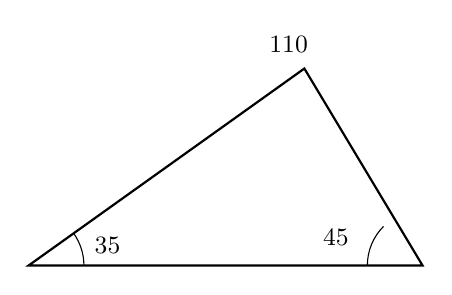
\begin{tikzpicture}[scale=1]
  \draw[thick] (0,0) -- (5,0) -- (3.5,2.5) -- cycle;
  \draw (0.7,0) arc[start angle=0,end angle=35,radius=0.7];
  \node at (1.0,0.25) {\small $35°$};
  \draw (4.3,0) arc[start angle=180,end angle=135,radius=0.7];
  \node at (3.9,0.35) {\small $45°$};
  \node at (3.3,2.8) {\small $110°$};
\end{tikzpicture}
\end{center}
\end{questionText}
\choiceA{Yes, because $35 + 45 + 110 = 190$}
\choiceB{Yes, because all angles are positive}
\choiceC{No, because the angles sum to $190°$ instead of $180°$}
\choiceD{No, because one angle is greater than $90°$}
\correctAnswer{C}
\explanation{$35 + 45 + 110 = 190 \neq 180$. Triangle angles must sum to exactly $180°$, so this triangle is not valid.}
\end{practiceQuestion}

\begin{practiceQuestion}{6-5-q29}{gsa}
\begin{questionText}
The diagram shows a cylinder with radius $4$ cm and height $9$ cm. A vertical cut is made through the center. Describe the cross-section and give its dimensions.

\begin{center}
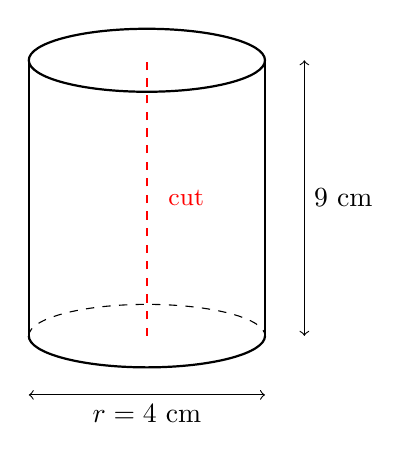
\begin{tikzpicture}[scale=0.5]
  % Cylinder
  \draw[thick] (-3,0) -- (-3,7);
  \draw[thick] (3,0) -- (3,7);
  \draw[thick] (-3,0) arc[start angle=180,end angle=360,x radius=3,y radius=0.8];
  \draw[dashed] (-3,0) arc[start angle=180,end angle=0,x radius=3,y radius=0.8];
  \draw[thick] (-3,7) arc[start angle=180,end angle=360,x radius=3,y radius=0.8];
  \draw[thick] (-3,7) arc[start angle=180,end angle=0,x radius=3,y radius=0.8];
  % Vertical cut line
  \draw[thick,red,dashed] (0,0) -- (0,7);
  \node[right,red] at (0.3,3.5) {\small cut};
  % Labels
  \draw[<->] (-3,-1.5) -- (3,-1.5);
  \node[below] at (0,-1.5) {$r = 4$ cm};
  \draw[<->] (4,0) -- (4,7);
  \node[right] at (4,3.5) {$9$ cm};
\end{tikzpicture}
\end{center}
\end{questionText}
\correctAnswer{Rectangle; $8$ cm by $9$ cm}
\explanation{A vertical cut through the center of a cylinder produces a rectangle. Width = diameter = $2 \times 4 = 8$ cm. Height = $9$ cm.}
\end{practiceQuestion}

\begin{practiceQuestion}{6-6-q30}{gsa}
\begin{questionText}
In the figure below, three angles meet on a straight line. Find the value of $x$ and the measure of each angle.

\begin{center}
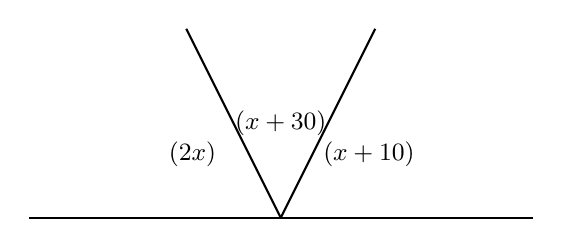
\begin{tikzpicture}[scale=0.8]
  \draw[thick] (-4,0) -- (4,0);
  \draw[thick] (0,0) -- (-1.5,3);
  \draw[thick] (0,0) -- (1.5,3);
  \node at (-1.4,1) {\small $(2x)°$};
  \node at (0,1.5) {\small $(x + 30)°$};
  \node at (1.4,1) {\small $(x + 10)°$};
\end{tikzpicture}
\end{center}
\end{questionText}
\correctAnswer{$x = 35$; angles are $70°$, $65°$, and $45°$}
\explanation{Angles on a line sum to $180°$: $2x + (x + 30) + (x + 10) = 180$. Combine: $4x + 40 = 180$. Solve: $4x = 140$, $x = 35$. Angles: $2(35) = 70°$, $35 + 30 = 65°$, $35 + 10 = 45°$. Check: $70 + 65 + 45 = 180°$ \checkmark.}
\end{practiceQuestion}

\begin{practiceQuestion}{6-7-q07}{mc}
\begin{questionText}
Point $F(0, -5)$ is reflected over the $x$-axis. What are the coordinates of $F'$?
\end{questionText}
\choiceA{$(0, 5)$}
\choiceB{$(0, -5)$}
\choiceC{$(5, 0)$}
\choiceD{$(-5, 0)$}
\correctAnswer{A}
\explanation{Over the $x$-axis: keep $x$, negate $y$. $(0, -5) \to (0, 5)$.}
\end{practiceQuestion}

\begin{practiceQuestion}{7-3-q03}{mc}
\begin{questionText}
A circle has a diameter of $12$ inches. What is its area? Use $\pi \approx 3.14$.
\end{questionText}
\choiceA{$37.68$ in$^2$}
\choiceB{$113.04$ in$^2$}
\choiceC{$452.16$ in$^2$}
\choiceD{$144$ in$^2$}
\correctAnswer{B}
\explanation{$r = 12 \div 2 = 6$ in. $A = \pi r^2 = 3.14 \times 36 = 113.04$ in$^2$.}
\end{practiceQuestion}

\begin{practiceQuestion}{7-4-q25}{sa}
\begin{questionText}
A trapezoidal garden has parallel sides of $8$ m and $12$ m, and a height of $5$ m. What is its area?
\end{questionText}
\correctAnswer{$50$ m$^2$}
\explanation{$A = \frac{1}{2}(b_1 + b_2) \times h = \frac{1}{2}(8 + 12) \times 5 = \frac{1}{2} \times 20 \times 5 = 50$ m$^2$.}
\end{practiceQuestion}

\begin{practiceQuestion}{7-5-q10}{mc}
\begin{questionText}
A cube has a surface area of $54$ cm$^2$. What is the area of one face?
\end{questionText}
\choiceA{$6$ cm$^2$}
\choiceB{$9$ cm$^2$}
\choiceC{$18$ cm$^2$}
\choiceD{$27$ cm$^2$}
\correctAnswer{B}
\explanation{A cube has $6$ identical faces. Area of one face $= 54 \div 6 = 9$ cm$^2$.}
\end{practiceQuestion}

\begin{practiceQuestion}{7-6-q25}{sa}
\begin{questionText}
Two rectangular prisms have the same base of $5$ cm by $4$ cm. Prism A is $6$ cm tall and Prism B is $9$ cm tall. What is the difference in their volumes?
\end{questionText}
\correctAnswer{$60$ cm$^3$}
\explanation{$V_A = 5 \times 4 \times 6 = 120$ cm$^3$. $V_B = 5 \times 4 \times 9 = 180$ cm$^3$. Difference: $180 - 120 = 60$ cm$^3$.}
\end{practiceQuestion}

\begin{practiceQuestion}{8-1-q07}{mc}
\begin{questionText}
Which of the following is an example of a biased sample?
\end{questionText}
\choiceA{Randomly selecting $50$ names from a hat containing all student names}
\choiceB{Using a random number generator to pick $30$ employees}
\choiceC{Asking every $10$th person who enters a store}
\choiceD{Surveying only members of the basketball team about school sports}
\correctAnswer{D}
\explanation{Basketball players have strong opinions about sports that may not represent the whole school.}
\end{practiceQuestion}

\begin{practiceQuestion}{8-3-q23}{sa}
\begin{questionText}
What does it mean when two box plots have a large gap between them on a number line?
\end{questionText}
\correctAnswer{The two groups have very different values with little or no overlap}
\explanation{A large gap indicates the groups' data ranges do not overlap much, suggesting a clear difference between the populations.}
\end{practiceQuestion}

\begin{practiceQuestion}{8-4-q19}{sa}
\begin{questionText}
Data: $30, 35, 40, 45, 50$. Find the mean and range.
\end{questionText}
\correctAnswer{Mean $= 40$; Range $= 20$}
\explanation{Mean: $\frac{30+35+40+45+50}{5} = \frac{200}{5} = 40$. Range: $50 - 30 = 20$.}
\end{practiceQuestion}

\begin{practiceQuestion}{8-7-q25}{sa}
\begin{questionText}
A double bar graph shows monthly book sales: Store A sold $120$ in March and $150$ in April. Store B sold $100$ in March and $180$ in April. Which store had a greater percent increase from March to April?
\end{questionText}
\correctAnswer{Store B ($80\%$ increase vs.\ $25\%$)}
\explanation{Store A: $\frac{150-120}{120} = \frac{30}{120} = 25\%$. Store B: $\frac{180-100}{100} = \frac{80}{100} = 80\%$. Store B had a greater percent increase.}
\end{practiceQuestion}

\begin{practiceQuestion}{9-4-q28}{gmc}
\begin{questionText}
Look at the two bags below. Which bag represents a uniform probability model for drawing a marble?

\begin{center}
\begin{tikzpicture}[scale=0.65]
  % Bag 1
  \draw[thick,rounded corners=8pt] (-3,-1.5) rectangle (0,1.5);
  \node[above,font=\bfseries] at (-1.5,1.5) {Bag 1};
  \fill[funRed] (-2.3,0.5) circle (0.3);
  \fill[funRed] (-1.5,0.5) circle (0.3);
  \fill[funBlue] (-0.7,0.5) circle (0.3);
  \fill[funBlue] (-2.3,-0.5) circle (0.3);
  \fill[funGreen] (-1.5,-0.5) circle (0.3);
  \fill[funGreen] (-0.7,-0.5) circle (0.3);
  % Bag 2
  \draw[thick,rounded corners=8pt] (1,-1.5) rectangle (4,1.5);
  \node[above,font=\bfseries] at (2.5,1.5) {Bag 2};
  \fill[funRed] (1.7,0.5) circle (0.3);
  \fill[funRed] (2.5,0.5) circle (0.3);
  \fill[funRed] (3.3,0.5) circle (0.3);
  \fill[funRed] (1.7,-0.5) circle (0.3);
  \fill[funBlue] (2.5,-0.5) circle (0.3);
  \fill[funGreen] (3.3,-0.5) circle (0.3);
\end{tikzpicture}
\end{center}
\end{questionText}
\choiceA{Bag 1 only}
\choiceB{Bag 2 only}
\choiceC{Both bags}
\choiceD{Neither bag}
\correctAnswer{A}
\explanation{Bag 1 has $2$ of each color ($2$ red, $2$ blue, $2$ green), so each color is equally likely — uniform. Bag 2 has $4$ red, $1$ blue, $1$ green — non-uniform.}
\end{practiceQuestion}

\begin{practiceQuestion}{9-6-q17}{mc}
\begin{questionText}
Two spinners are spun. Spinner 1 has sections $\{1, 2, 3\}$ and Spinner 2 has sections $\{A, B\}$. What is the probability of getting $2$ and $A$?
\end{questionText}
\choiceA{$\frac{1}{3}$}
\choiceB{$\frac{1}{5}$}
\choiceC{$\frac{1}{6}$}
\choiceD{$\frac{2}{6}$}
\correctAnswer{C}
\explanation{$P(2) = \frac{1}{3}$, $P(A) = \frac{1}{2}$. $P = \frac{1}{3} \times \frac{1}{2} = \frac{1}{6}$.}
\end{practiceQuestion}

\begin{practiceQuestion}{9-7-q19}{sa}
\begin{questionText}
A simulation uses a coin flip ($50\%$ chance) to model whether it rains on a given day. In $30$ trials, rain occurs $16$ times. What is the experimental probability of rain?
\end{questionText}
\correctAnswer{$\frac{16}{30}$}
\explanation{$P = \frac{16}{30} \approx 0.533$.}
\end{practiceQuestion}
